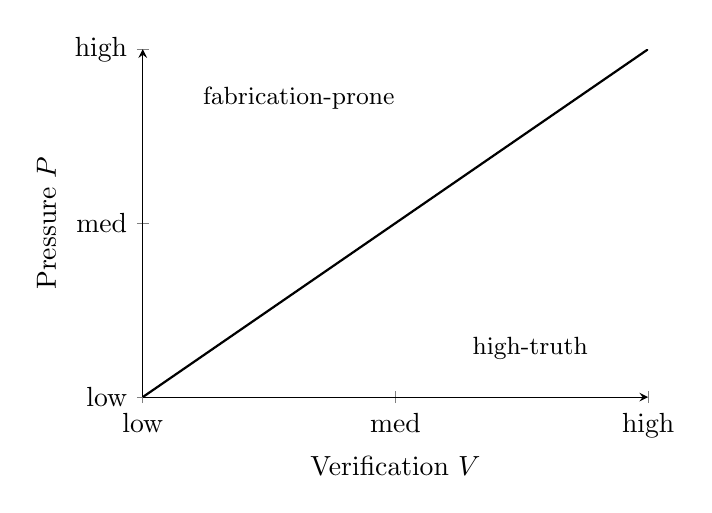
\begin{tikzpicture}
\begin{axis}[
    width=8cm,
    height=6cm,
    xlabel={Verification $V$},
    ylabel={Pressure $P$},
    xmin=0, xmax=1,
    ymin=0, ymax=1,
    axis lines=left,
    xtick={0,0.5,1},
    ytick={0,0.5,1},
    xticklabels={low,med,high},
    yticklabels={low,med,high}
]

% Boundary curve (illustrative): high-truth region where V > P
\addplot[domain=0:1, thick, black] {x};

\node[anchor=south west, font=\small] at (axis cs:0.1,0.8)
  {fabrication-prone};

\node[anchor=north east, font=\small] at (axis cs:0.9,0.2)
  {high-truth};

\end{axis}
\end{tikzpicture}
